\section{Repeated Bayesian extension (BR-PEG)}
\label{app:bayesian}

The main paper analyses a one-shot full-information game. We have so far
left aside two natural extensions: (i) repetition across rounds, and (ii)
private knowledge of the players' utility weights. Both extensions have a
clean home in the literature on repeated games with incomplete
information, and this appendix sketches how the PEG specialises to a
standard template in that line of work. We define the resulting game
formally (the \emph{Bayesian Repeated PEG}, BR-PEG) and report a small
simulation that shows the qualitative behaviour the existing theory
predicts.

\paragraph{Position in the literature.}
The classical framework for a repeated zero-sum game with one-sided
private information is \citet{aumann1995repeated}; their central question
is how the informed player should manage the information it reveals
through its actions. A closely related strand, motivated by security
applications, considers a leader who commits to a strategy each round and
a follower of unknown type who best-responds; the leader observes the
follower's response and refines its belief over the follower's payoff
function~\cite{letchford2009learning, blum2014learning,
balcan2015commitment}. Theoretical guarantees from
\citet{kalai1993rational} show that, under a mild absolute-continuity
condition on the prior, rational Bayesian updating in such games leads to
play that converges to a Nash equilibrium of the repeated game. A
separate but related body of work studies privacy as a transacted good
with heterogeneous private valuations~\cite{ghosh2011selling}, and
sender-receiver problems in which a privileged party commits to an
information structure~\cite{kamenica2011bayesian}; both are conceptually
close but solve different mechanism-design problems.

The BR-PEG is a direct instance of the Stackelberg-learning template of
\citet{letchford2009learning, blum2014learning, balcan2015commitment}
applied to the iDP mechanism of \cref{def:sampling-idp}. The leader is
the (malicious) player M who commits to a budget $\eps_M$ and a sample
count $n_M$ each round; the follower is the (myopic) player H who
best-responds with $\eps_H$ given their private type $\theta_H = (B_H,
C_H)$; M observes $(\eps_H, u_H)$ and Bayes-updates a posterior over
$\theta_H$. The differences from the standard template are minor: the
follower's action space is the continuous-ish interval
$[\eps^{\min}, \eps^{\max}]$ rather than a discrete set of attack
targets, and the per-round payoff is delivered by the iDP mechanism
rather than by a tabular game.

\paragraph{The game.}
Two players, H (honest) and M (malicious). H has a private type
$\theta_H = (B_H, C_H, n_H)$ drawn from a finite known set $\Theta$ at
$t=0$; M does not know $\theta_H$ but knows $\Theta$. Per round $t \in
\{1,\dots,T\}$:
\begin{itemize}
\item M observes the history $\mathcal{H}_{t-1}$ and picks
$(\eps_M^t, n_M^t)$.
\item H observes $(\eps_M^t, n_M^t)$ and best-responds with the
$\eps_H^t \in \mathcal{A}$ that maximises its one-shot utility
$u_H = B_H V(\sigma) - C_H A_H$ given $\theta_H$.
\item The mechanism returns $(\sigma^t, p_H^t, p_M^t, A_H^t, A_M^t)$.
\item The pair $(\eps_H^t, u_H^t)$ becomes public; M Bayes-updates its
posterior over $\theta_H$.
\item H accrues $u_H^t$; M accrues $A_H^t$ (M is malicious---it wants
H's vulnerability up).
\end{itemize}
M's total score is $\sum_t A_H^t$. The strategic content is the
identification problem: by observing how H's $\eps_H^t$ responds to M's
own choices, M can narrow down $\theta_H$ and then exploit that knowledge
in the remaining rounds. The framework is a one-sided
incomplete-information repeated game in the sense of
\citet{aumann1995repeated} but with the informed player myopic, which
reduces it to the Stackelberg-learning instance of
\citet{letchford2009learning}.

\paragraph{Simulation.}
We run a small instance to confirm the qualitative behaviour the existing
theory predicts. H's true type is $(B_H, C_H) = (2, 1)$; M's prior is
uniform over $\Theta = \{(0.5, 1), (1, 1), (2, 1)\}$. All other
parameters are the canonical ones of \cref{sec:experiments}, with the
two players' group sizes fixed at $n_H = n_M = 5000$. We compare three
M strategies: a benign constant $\eps_M = 64$ (a baseline that should
produce negligible $A_H$), a naive constant $\eps_M = 1$ (the
fixed-action attack of \cref{sec:C4}), and a posterior-greedy Bayesian
policy that picks the $\eps_M$ on the grid maximising the expected next-
round $A_H$ under M's current posterior.

\Cref{fig:bayesian} shows the result. M's posterior locks onto H's true
type within two to three rounds in all three regimes; the strategic
question is what M does once it has identified $\theta_H$. The benign
baseline holds $A_H$ flat at $0.01$, and the naive attack holds it at
$0.22$. The Bayesian-greedy attack identifies the true type in one round
and then plays $\eps_M \approx 3.1$ for the remaining rounds, eliciting
$\eps_H \approx 19$ from H and delivering a per-round $A_H \approx 0.45$
---roughly twice the naive attack and around fifty times the benign
baseline. The optimal adversarial budget is therefore \emph{not} the
minimum: M's gain comes not from forcing $\sigma$ down but from drawing
out a more exposing best response from H, a manoeuvre that requires
knowing H's type and is opened up precisely by the Bayesian updating.
This matches the intuition from the Stackelberg-learning
literature~\cite{letchford2009learning, blum2014learning}, in which a
leader equipped with type knowledge does strictly better than one
committed to a fixed strategy.

\begin{figure*}[!t]
\centering
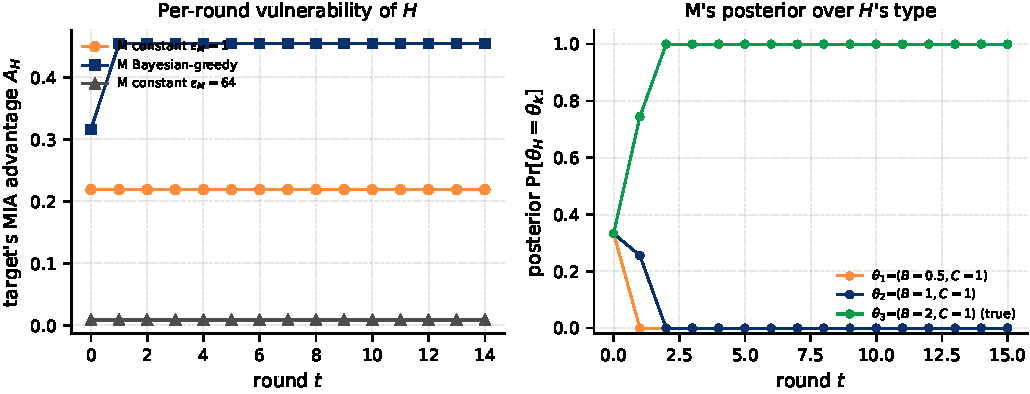
\includegraphics[width=0.95\linewidth]{figures/fig_bayesian.pdf}
\caption{\textbf{BR-PEG demo.} Left: per-round realised MIA advantage
$A_H$ of the honest player under three M policies. Right: M's posterior
over H's type under the Bayesian-greedy policy; the posterior collapses
to the true type within two rounds.}
\label{fig:bayesian}
\end{figure*}

\paragraph{What this leaves open.}
The simulation is illustrative rather than exhaustive. Two technical
points sit just outside the scope of this paper but are natural follow-
ups. The first is the case where H is also strategic across rounds
(a fully two-sided repeated game in the sense of
\citet{aumann1995repeated}), in which H would manage what it reveals
through its action sequence. The second is regret-bound analysis along
the lines of \citet{balcan2015commitment}: how many rounds does M need
before its per-round $A_H$ is within $\varepsilon$ of the
full-information optimum? Both extensions are well-studied in the
Stackelberg-learning literature; we have not pursued them here in order
to keep the focus on the one-shot phenomenology, but the framework above
slots into either with no further modification.
